% =====================================================================
%  FraudLens - Methodology block diagram
%  Compile:  pdflatex methodology.tex
%  Output :  methodology.pdf  (crop-free, ready to insert into PowerPoint)
%  To get a PNG:  pdftoppm -r 400 -png methodology.pdf methodology
% =====================================================================
\documentclass[border=6pt]{standalone}

\usepackage[T1]{fontenc}
\usepackage{amsmath}
\usepackage{tikz}
\usetikzlibrary{arrows.meta, positioning, calc, shapes.geometric}
\hyphenpenalty=10000 \exhyphenpenalty=10000

% ---- palette -------------------------------------------------------
\definecolor{hiFill}{HTML}{E6E6F7}   % lavender block fill
\definecolor{hiLine}{HTML}{2A2A8C}   % deep blue/purple stroke
\definecolor{inkCol}{HTML}{111111}

\begin{document}
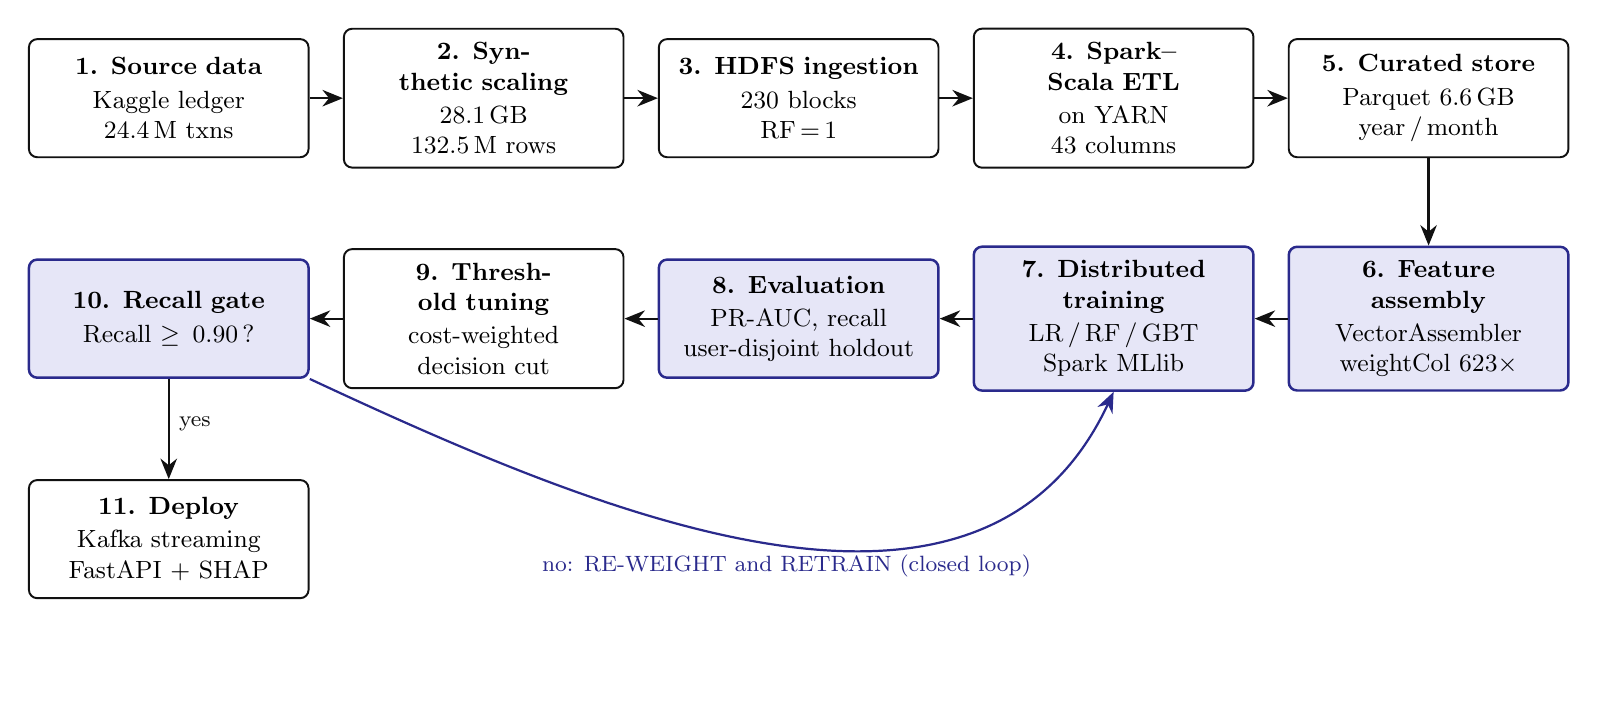
\begin{tikzpicture}[
  font=\small,
  node distance=0pt,
  % ---- plain block ----
  blk/.style={
    draw=inkCol, line width=0.7pt, rounded corners=3pt,
    fill=white, align=center, inner sep=5pt,
    text width=32mm, minimum height=15mm
  },
  % ---- highlighted block ----
  hblk/.style={
    blk, draw=hiLine, line width=0.9pt, fill=hiFill
  },
  % ---- arrows ----
  ar/.style={-{Stealth[length=2.6mm,width=2.1mm]}, line width=0.8pt, inkCol},
  loop/.style={-{Stealth[length=2.6mm,width=2.1mm]}, line width=0.8pt, hiLine}
]

% ======================= geometry ===================================
\def\cx{40mm}   % column pitch
\def\ry{28mm}   % row pitch

% ======================= ROW 1 (left -> right) ======================
\node[blk] (n1) at (0*\cx, 0)      {\textbf{1. Source data}\\[1pt]Kaggle ledger\\24.4\,M txns};
\node[blk] (n2) at (1*\cx, 0)      {\textbf{2. Synthetic scaling}\\[1pt]28.1\,GB\\132.5\,M rows};
\node[blk] (n3) at (2*\cx, 0)      {\textbf{3. HDFS ingestion}\\[1pt]230 blocks\\RF\,=\,1};
\node[blk] (n4) at (3*\cx, 0)      {\textbf{4. Spark--Scala ETL}\\[1pt]on YARN\\43 columns};
\node[blk] (n5) at (4*\cx, 0)      {\textbf{5. Curated store}\\[1pt]Parquet 6.6\,GB\\year\,/\,month};

\draw[ar] (n1) -- (n2);
\draw[ar] (n2) -- (n3);
\draw[ar] (n3) -- (n4);
\draw[ar] (n4) -- (n5);

% ======================= ROW 2 (right -> left) ======================
\node[hblk] (n6)  at (4*\cx, -\ry) {\textbf{6. Feature assembly}\\[1pt]VectorAssembler\\weightCol 623$\times$};
\node[hblk] (n7)  at (3*\cx, -\ry) {\textbf{7. Distributed training}\\[1pt]LR\,/\,RF\,/\,GBT\\Spark MLlib};
\node[hblk] (n8)  at (2*\cx, -\ry) {\textbf{8. Evaluation}\\[1pt]PR-AUC, recall\\user-disjoint holdout};
\node[blk]  (n9)  at (1*\cx, -\ry) {\textbf{9. Threshold tuning}\\[1pt]cost-weighted\\decision cut};
\node[hblk] (n10) at (0*\cx, -\ry) {\textbf{10. Recall gate}\\[1pt]Recall $\geq 0.90$\,?};

\draw[ar] (n5) -- (n6);
\draw[ar] (n6) -- (n7);
\draw[ar] (n7) -- (n8);
\draw[ar] (n8) -- (n9);
\draw[ar] (n9) -- (n10);

% ======================= ACCEPT branch ==============================
\node[blk] (acc) at (0*\cx, -2*\ry)
  {\textbf{11. Deploy}\\[1pt]Kafka streaming\\FastAPI + SHAP};

\draw[ar] (n10) -- node[right, pos=0.45, font=\footnotesize] {yes} (acc);

% ======================= closed-loop feedback =======================
\draw[loop] (n10.south east)
  to[out=-25, in=-115] node[below, pos=0.52, font=\footnotesize, hiLine]
  {no: RE-WEIGHT and RETRAIN (closed loop)} (n7.south);

\end{tikzpicture}
\end{document}
